% Options for packages loaded elsewhere
\PassOptionsToPackage{unicode}{hyperref}
\PassOptionsToPackage{hyphens}{url}
%
\documentclass[
]{article}
\usepackage{lmodern}
\usepackage{amssymb,amsmath}
\usepackage{ifxetex,ifluatex}
\ifnum 0\ifxetex 1\fi\ifluatex 1\fi=0 % if pdftex
  \usepackage[T1]{fontenc}
  \usepackage[utf8]{inputenc}
  \usepackage{textcomp} % provide euro and other symbols
\else % if luatex or xetex
  \usepackage{unicode-math}
  \defaultfontfeatures{Scale=MatchLowercase}
  \defaultfontfeatures[\rmfamily]{Ligatures=TeX,Scale=1}
\fi
% Use upquote if available, for straight quotes in verbatim environments
\IfFileExists{upquote.sty}{\usepackage{upquote}}{}
\IfFileExists{microtype.sty}{% use microtype if available
  \usepackage[]{microtype}
  \UseMicrotypeSet[protrusion]{basicmath} % disable protrusion for tt fonts
}{}
\makeatletter
\@ifundefined{KOMAClassName}{% if non-KOMA class
  \IfFileExists{parskip.sty}{%
    \usepackage{parskip}
  }{% else
    \setlength{\parindent}{0pt}
    \setlength{\parskip}{6pt plus 2pt minus 1pt}}
}{% if KOMA class
  \KOMAoptions{parskip=half}}
\makeatother
\usepackage{xcolor}
\IfFileExists{xurl.sty}{\usepackage{xurl}}{} % add URL line breaks if available
\IfFileExists{bookmark.sty}{\usepackage{bookmark}}{\usepackage{hyperref}}
\hypersetup{
  pdftitle={Appendix},
  pdfauthor={Author names redacted},
  hidelinks,
  pdfcreator={LaTeX via pandoc}}
\urlstyle{same} % disable monospaced font for URLs
\usepackage[margin=1in]{geometry}
\usepackage{graphicx}
\makeatletter
\def\maxwidth{\ifdim\Gin@nat@width>\linewidth\linewidth\else\Gin@nat@width\fi}
\def\maxheight{\ifdim\Gin@nat@height>\textheight\textheight\else\Gin@nat@height\fi}
\makeatother
% Scale images if necessary, so that they will not overflow the page
% margins by default, and it is still possible to overwrite the defaults
% using explicit options in \includegraphics[width, height, ...]{}
\setkeys{Gin}{width=\maxwidth,height=\maxheight,keepaspectratio}
% Set default figure placement to htbp
\makeatletter
\def\fps@figure{htbp}
\makeatother
\setlength{\emergencystretch}{3em} % prevent overfull lines
\providecommand{\tightlist}{%
  \setlength{\itemsep}{0pt}\setlength{\parskip}{0pt}}
\setcounter{secnumdepth}{-\maxdimen} % remove section numbering

\title{Appendix}
\author{Author names redacted}
\date{2020-11-12}

\begin{document}
\maketitle

{
\setcounter{tocdepth}{5}
\tableofcontents
}
This appendix provides supplemental information about the dataset of
Russian gray zone campaigns introduced in the accompanying paper ``After
Deterrence: Explaining Conflict Short of War''

\hypertarget{formal-model}{%
\section{Formal Model}\label{formal-model}}

\hypertarget{formal-statement-of-assumptions}{%
\subsection{Formal statement of
assumptions}\label{formal-statement-of-assumptions}}

First, we express the assumption that the kinks in the P function are
never activated in equilibrium. Letting \(\tilde{g_{C}}\) and
\(\tilde{g_{D}}\) denote the optimal levels selected by C and D
conditional on the actors selecting into gray zone conflict (these are
defined below), when Assumption 1 holds, the ``min-max'\,' statements in
the \(P\) function will never be relevant to analysis.

\textbf{\textit{Assumption 1}}\textit{: In equilibrium, $\rho_{0}<P(\tilde{g_{C}},\tilde{g_{D}})<1$.}\footnote{Based on the optimal $\tilde{g_{C}}$ and $\tilde{g_{D}}$ (solved below), this condition amounts to $\frac{\theta}{2\beta_{C}}-\frac{1}{2\beta_{D}}>0$ and $\frac{1}{\beta_{D}}-\frac{\theta}{\beta_{C}}-2\rho_{0}+2>0$ if $\frac{\theta}{2\beta_{C}}<\rho_{W}-\rho_{0}+\kappa_{D}+\frac{1}{4\beta_{D}}$, and $\rho_{W}-\rho_{0}+\kappa_{D}-\frac{1}{4\beta_{D}}>0$ and $\frac{1}{\beta_{D}}-4\left(\kappa_{D}-1+\rho_{W}\right)>0$ if $\rho_{W}-\rho_{0}+\kappa_{D}+\frac{1}{4\beta_{D}}\leq\frac{\theta}{2\beta_{C}}$.}

Second, we express the assumption that if C's resolve increases, C
becomes more willing to go to war over using gray zone conflict. As some
intuition, conditional on gray zone conflict occurring, C selects one of
two values for \(r\). For the first value, the selected \(r\) will be
the largest possible \(r\) that is tailored to keep D from going to war.
I call this \(\hat{g_{C}}\). For the second value, the selected
\(g_{C}\) will be based on C's own resolve and represents the solution
to C's internal optimization problem or C's internal efficiency. I call
this
\(\check{g_{C}}\).\footnote{Intuitively, $\tilde{g_{C}}$ is defined by $\tilde{g_{C}}=min\{\hat{g_{C}},\check{g_{C}}\}$.}
For C's utility from war to be increasing in \(\theta\) at a faster rate
than the utility from gray zone conflict, we must consider both values
of \(g_{C}\).

\textbf{\textit{ Assumption 2:}}\textit{ The following must hold: $\frac{d}{d\theta}\left[\theta\rho_{W}-\kappa_{D}-\left(\theta P(\hat{g_{C}},\tilde{g_{D}})-\beta(\tilde{g_{D}})^{2}\right)\right]>0$ }

\textit{ and $\frac{d}{d\theta}\left[\theta\rho_{W}-\kappa_{D}-\left(\theta P(\check{g_{C}},\tilde{g_{D}})-\beta(\tilde{g_{D}})^{2}\right)\right]>0$.}\footnote{Based on the optimal $\hat{g_{C}}$, $\check{g_{C}}$, and $\tilde{g_{D}}$ (solved below), this condition amounts to $\rho_{W}-\rho_{0}+\frac{1}{2\beta_{D}}-\frac{\theta}{2\beta_{C}}>0$ and $-\kappa_{D}+\frac{1}{4\beta_{D}}>0$. }

\hypertarget{proving-proposition-1}{%
\subsection{Proving Proposition 1}\label{proving-proposition-1}}

\hypertarget{equilibrium-intuition}{%
\subsubsection{Equilibrium Intuition}\label{equilibrium-intuition}}

Outside of gray zone conflict, C will prefer the status quo to initially
going to war when \begin{align*}
\theta\rho_{0}\geq & \theta\rho_{W}-\kappa_{C}
\end{align*} or \begin{align*}
\theta\leq & \frac{\kappa_{C}}{\rho_{W}-\rho_{0}}.
\end{align*} Here I discuss the intuition of the equilibrium in the
paper. Assume for now that C is optimally selecting a \(g_{C}^{*}\) such
that the game ends in gray zone conflict (in other words assume that
\(w_{R}^{*}=0\) and \(g_{C}^{*}\geq0\)). Also assume that D selects an
optimal \(g_{D}^{*}\) such that \(g_{D}^{*}\leq g_{C}^{*}\) (this will
be borne out by Assumption 1). D selects \(g_{D}^{*}\) characterized by
\begin{align*}
g_{D}^{*}\in & argmax_{g_{D}\geq0}\left\{ 1-\rho_{0}-g_{C}+g_{D}-\beta_{D}g_{D}^{2}\right\} .
\end{align*} I take first-order conditions with respect to \(g_{D}\) and
solve the expression above to identify the optimal level of D's gray
zone response \(g_{D}^{*}\). This unique value is \begin{align*}
g_{D}^{*}= & \frac{1}{2\beta_{D}}.
\end{align*} Using the expression for \(g_{D}^{*}\), D's utility in
terms of the selected \(g_{C}^{*}\) is
\(U_{D}=1-\rho_{0}-g_{C}^{*}+\frac{1}{4\beta_{D}}\). \textbackslash{}
\textbackslash{} I can then begin considering C's utility. There are two
things to consider. First, it could be that C will select an optimal
\(g_{C}^{*}\) that is constrained by D's willingness to go to war.
Essentially, if
\(g_{C}>\rho_{W}-\rho_{0}+\kappa_{D}+\frac{1}{4\beta_{D}}\), then D's
utility from war is greater than D's utility from gray zone conflict;
thus, if C wants to remain in gray zone conflict and will be constrained
by D's deterrent threat, C will select \(\hat{g_{C}}\), where
\(\hat{g_{C}}\) is the greatest \(g_{C}\) that would make D indifferent
between gray zone conflict and war, or \begin{align*}
\hat{g_{C}} & =\rho_{W}-\rho_{0}+\kappa_{D}+\frac{1}{4\beta_{D}}.
\end{align*} Second C may select an optimal \(g_{C}^{*}\) that is
constrained by their own internal costs. When this is the case, C will
select \(\check{g_{C}}\), defined by the optimization \begin{align*}
\check{g_{C}}\in & argmax_{g_{C}\geq0}\left\{ \theta\left(\rho_{0}+g_{C}-\frac{1}{2\beta_{D}}\right)-\beta_{C}g_{C}\right\} ,
\end{align*} which yields \begin{align*}
\check{g_{C}} & =\frac{\theta}{2\beta_{C}}.
\end{align*} Before discussing the true behavior, I want to highlight
two things that do not happen. First, note that C will never select an
\(g_{C}\) that provokes D to go to war in the final stage, because this
is strictly worse than initially going to war. Second, note that C will
never select into gray zone conflict (i.e.~set \(w_{R}=0\) and
\(g_{C}^{*}>0\)) if \(g_{D}^{*}\) as defined above is greater than
\(g_{C}^{*}\) because C could do strictly better not paying the costs of
war and selecting into the status quo (\(g_{C}^{*}=0\)).\textbackslash{}
\textbackslash{} With this is place, I can say that if C optimally
selects into gray zone conflict, C will select
\(g_{C}^{*}=\tilde{g_{C}}\), where \begin{align*}
\tilde{g_{C}}= & min\left\{ \hat{g_{C}},\check{g_{C}}\right\} .
\end{align*} I've characterized what happens withing gray zone conflict.
I now need to describe how the game optimally plays out across the
possibility of selecting into the status quo, war (at the onset;
\(w_{A}=1\)), or gray zone conflict. Because C moves first, this is
ultimately C's choice. I can calculate C's decision within the two cases
of gray zone conflict:\textbackslash{} \textbackslash{} First, I
consider the case when
\(\frac{\theta}{2\beta_{C}}\geq\rho_{W}-\rho_{0}+\kappa_{D}+\frac{1}{4\beta_{D}}\).
This condition implies that the selected gray zone conflict will be
constrained by D's deterrent threat and not C's internal costs. So, if C
selects into gray zone conflict, C will select
\(g_{C}^{*}=\hat{g_{C}}=\rho_{W}-\rho_{0}+\kappa_{D}+\frac{1}{4\beta_{D}}\).
I can then express C's behavior in terms of \(\theta\). C prefers the
status quo to gray zone conflict when \begin{align*}
\theta\rho_{0}\geq & \theta\left(\rho_{W}+\kappa_{D}-\frac{1}{4\beta_{D}}\right)-\beta_{C}\left(\rho_{W}-\rho_{0}+\kappa_{D}+\frac{1}{4\beta_{D}}\right)^{2}
\end{align*} or \begin{align*}
\theta\leq & \frac{\beta_{C}\left(\rho_{W}-\rho_{0}+\kappa_{D}+\frac{1}{4\beta_{D}}\right)^{2}}{\left(\rho_{W}-\rho_{0}+\kappa_{D}-\frac{1}{4\beta_{D}}\right)}.
\end{align*} Note that the above derivation relies on
\(\rho_{W}-\rho_{0}+\kappa_{D}-\frac{1}{4\beta_{D}}>0\), lest the
inequality sign would flip. This is assumed by Assumption
1.\textbackslash{} \textbackslash{} Next, C prefers war to gray zone
conflict when

\begin{align*}
\theta\rho_{W}-\kappa_{C}> & \theta\left(\rho_{W}+\kappa_{D}-\frac{1}{4\beta_{D}}\right)-\beta_{C}\left(\rho_{W}-\rho_{0}+\kappa_{D}+\frac{1}{4\beta_{D}}\right)^{2}
\end{align*} or \begin{align*}
\theta> & \frac{\kappa_{C}-\beta_{C}\left(\rho_{W}-\rho_{0}+\kappa_{D}+\frac{1}{4\beta_{D}}\right)^{2}}{\frac{1}{4\beta_{D}}-\kappa_{D}}.
\end{align*} Note that the above derivation relies on
\(\frac{1}{4\beta_{D}}-\kappa_{D}>0\), lest the inequality sign would
flip. this is assumed by Assumption 2. \textbackslash{} \textbackslash{}
Next, I assume
\(\frac{\theta}{2\beta_{C}}<\rho_{W}-\rho_{0}+\kappa_{D}+\frac{1}{4\beta_{D}}\).
This condition implies that the selected gray zone conflict will be
constrained by C's internal costs and not D's deterrent threat. So, if C
selects into gray zone conflict, C will select
\(g_{C}^{*}=\check{g_{C}}=\frac{\theta}{2\beta_{C}}\). I can then
express C's behavior in terms of \(\theta\). C prefers the status quo to
gray zone conflict when \begin{align*}
\theta\rho_{0}\geq & \theta\rho_{0}+\frac{\theta^{2}}{4\beta_{C}}-\frac{\theta}{2\beta_{D}}
\end{align*} or \begin{align*}
0\geq & \theta\left(\frac{\theta}{4\beta_{C}}-\frac{1}{2\beta_{D}}\right).
\end{align*} Next, C prefers war to gray zone conflict when
\begin{align*}
\theta\rho_{W}-\kappa_{C}> & \theta\rho_{0}+\frac{\theta^{2}}{4\beta_{C}}-\frac{\theta}{2\beta_{D}}
\end{align*} or \begin{align*}
\theta> & \frac{\kappa_{C}}{\rho_{W}-\rho_{0}-\frac{\theta}{4\beta_{C}}+\frac{1}{2\beta_{D}}}.
\end{align*} Note that the above derivation relies on
\(\rho_{W}-\rho_{0}-\frac{\theta}{4\beta_{C}}+\frac{1}{2\beta_{D}}>0\),
lest the inequality sign would flip. This is implied by Assumption 2.
\textbackslash{} \textbackslash{} With all of this defined, we can
characterize C's strategy in terms of \(\theta\); as \(\theta\)
increases, C prefers more degrees of conflict (i.e.~larger
\(g_{C}^{*}'s\) or war) to get what they want.

\hypertarget{equilibrium-behavior}{%
\subsubsection{Equilibrium Behavior}\label{equilibrium-behavior}}

Proposition 1A and the text below contains a more complete discussion on
the equilibrium behavior characterized in Proposition 1.
\textbackslash{} \textbackslash{}
\textbf{\textit{Proposition 1A:}}\textit{ In equilibrium, the game will play out in the following manner.}\textbackslash{}
\textbackslash{}
\textit{Case 1, $\frac{\theta}{2\beta_{C}}\geq\rho_{W}-\rho_{0}+\kappa_{D}+\frac{1}{4\beta_{D}}$:}

\begin{itemize}
\item \textit{1.A. If $\theta\leq\frac{\beta_{C}\left(\rho_{W}-\rho_{0}+\kappa_{D}+\frac{1}{4\beta_{D}}\right)^{2}}{\left(\rho_{W}-\rho_{0}+\kappa_{D}-\frac{1}{4\beta_{D}}\right)}$ and $\theta\leq\frac{\kappa_{C}}{\rho_{W}-\rho_{0}}$, then C accepts the status quo. C selects $w_{R}^{*}=0$ and $g_{C}^{*}=0$, and D selects $w_{D}^{*}=0$ and $g_{D}^{*}=0$. Payoffs are $U_{D}=1-\rho_{0}$ and $U_{C}=\theta\rho_{0}.$} 
\item \textit{1.B. If $\theta>\frac{\kappa_{C}-\beta_{C}\left(\rho_{W}-\rho_{0}+\kappa_{D}+\frac{1}{4\beta_{D}}\right)^{2}}{\frac{1}{4\beta_{D}}-\kappa_{D}}$ and $\theta>\frac{\kappa_{C}}{\rho_{W}-\rho_{0}}$, then C declares war. C selects $w_{R}^{*}=1$, and payoffs are $U_{D}=1-\rho_{W}-\kappa_{D}$ and $U_{C}=\theta\rho_{W}-\kappa_{A}$.} 
\item \textit{1.C. Otherwise, the game end in gray zone conflict where }C's\textit{ limited challenge is constrained by D's deterrent threat. C selects $w_{R}^{*}=0$ and $g_{C}^{*}=\rho_{W}-\rho_{0}+\kappa_{D}+\frac{1}{4\beta_{D}}$, and D selects $w_{D}^{*}=0$ and $g_{D}^{*}=\frac{1}{2\beta_{D}}$. Payoffs are $U_{D}=1-\rho_{W}-\kappa_{D}$ and $U_{C}=\theta\left(\rho_{W}+\kappa_{D}-\frac{1}{4\beta_{D}}\right)-\beta_{C}\left(\rho_{W}-\rho_{0}+\kappa_{D}+\frac{1}{4\beta_{D}}\right)^{2}.$} 
\end{itemize}

\textit{Case 2, $\frac{\theta}{2\beta_{C}}<\rho_{W}-\rho_{0}+\kappa_{D}+\frac{1}{4\beta_{D}}$:}

\begin{itemize}
\item \textit{2.A. If $\theta\leq\frac{2\beta_{C}}{\beta_{D}}$ and $\theta\leq\frac{\kappa_{C}}{\rho_{W}-\rho_{0}}$, then C accepts the status quo. C selects $w_{R}^{*}=0$ and $g_{C}^{*}=0$, and D selects $w_{D}^{*}=0$ and $g_{D}^{*}=0$. Payoffs are $U_{D}=1-\rho_{0}$ and $U_{C}=\theta\rho_{0}.$} 
\item \textit{2.B. If $\theta>\frac{\kappa_{C}}{\rho_{W}-\rho_{0}-\frac{\theta}{4\beta_{C}}+\frac{1}{2\beta_{D}}}$ and $\theta>\frac{\kappa_{C}}{\rho_{W}-\rho_{0}}$, then C declares war. C sets $w_{R}^{*}=1$. Payoffs are $U_{D}=1-\rho_{W}-\kappa_{D}$ and $U_{C}=\theta\rho_{W}-\kappa_{A}$.} 
\item \textit{2.C. Otherwise, the game will end in gray zone conflict where }C's\textit{ limited challenge is constrained by }C's\textit{ internal efficiency. C selects $w_{R}^{*}=0$ and $g_{C}^{*}=\frac{\theta}{2\beta_{C}}$, and D selects $w_{D}^{*}=0$ and $g_{D}^{*}=\frac{1}{2\beta_{D}}$. Payoffs are $U_{D}=1-\rho_{0}-\frac{\theta}{2\beta_{C}}+\frac{1}{4\beta_{D}},$ and $U_{C}=\theta\rho_{0}+\frac{\theta^{2}}{4\beta_{C}}-\frac{\theta}{2\beta_{D}}.$} 
\end{itemize}

Working backwards, D will declare war for all
\(g_{C}>\rho_{W}-\rho_{0}+\kappa_{D}+\frac{1}{4\beta_{D}}\). If
\(g_{C}\leq\rho_{W}-\rho_{0}+\kappa_{D}+\frac{1}{4\beta_{D}}\), D will
select \$g\_\{D\}=min\left\{ \frac{1}{2\beta_{D}},g\_\{C\}\right\} \$.
When \(g_{D}=\frac{1}{2\beta_{D}}\), D is selecting their optimal level
of gray zone response based on their internal optimization. When
\(g_{D}=g_{C}\), it implies that D would be willing to select a greater
gray zone response, but does not need to, essentially driving the
political impact of C's limited challenges back to zero (at cost).

\hypertarget{observation-1-discussion}{%
\subsection{Observation 1 Discussion}\label{observation-1-discussion}}

Assume for now the parameters are such that the Case 1.C. conditions
hold, and consider what happens when \(\kappa_{D}\) decreases. Because
here C selects the greatest level of limited challenges that will not
provoke D to war, C's selected \(g_{C}^{*}\) is a decreasing function of
\(\kappa_{D}\); therefore, because \(g_{D}^{*}\) is fixed, the final
extent of gray zone conflict will be less. Of course, the analysis does
not stop there. Improvements in D's willingness to go to war constrain
how useful gray zone conflict is to R, and, within case 1.C., C's
utility is decreasing in
\(-\kappa_{D}\).\footnote{This follows from $\frac{d}{d\kappa_{D}}U_{D}=\theta-2\beta_{C}\left[\rho_{W}-\rho_{0}+\kappa_{D}+\frac{1}{4\beta_{D}}\right]>0$, as determined by the conditions for Case 1 to hold.}
Thus, if \(\kappa_{D}\) becomes small enough, C will leave gray zone
conflict and instead select into either accepting the status quo
(entering into case 1A) or going to war (entering into Case 1B).
Additionally, it is worthwhile noting that as \(\kappa_{D}\) decreases,
the condition that selects into Case 1 (over Case 2) has more slack,
implying that improvements in D's willingness to go to war will keep D
in within Case 1.\textbackslash{} \textbackslash{} Now assume the
parameters are such that the Case 2.C. conditions hold, and consider
what happens when \(\kappa_{D}\) decreases. Note that this will not
change the selected \(g_{C}^{*}\) here, but it could break the
inequality
\(\frac{\theta}{2\beta_{C}}<\rho_{W}-\rho_{0}+\kappa_{D}+\frac{1}{4\beta_{D}}\)
that determines whether the equilibrium is defined in Case 1 or Case 2.
thus, for a small enough \(\kappa_{D}\), the conditions for Case 2 will
break and the conditions for Case 1 will hold. When this happens, either
the selected \(g_{C}^{*}\) is increasing in \(\kappa_{D}\) (Case 1.C.)
or gray zone conflict is not selected (Case 1.A. or 1.B.).

\hypertarget{extension-1-endogenous-beta_d}{%
\subsection{\texorpdfstring{Extension 1: Endogenous
\(\beta_{D}\)\}}{Extension 1: Endogenous \textbackslash beta\_\{D\}\}}}\label{extension-1-endogenous-beta_d}}

In the model in the paper, I treated D's gray zone efficiency
\(\beta_{D}\) as exogenous. In some special cases or under some
conditions, this may be too strong an assumption. In this section, I
characterize an equilibrium for the game when D can have complete
flexibility in selecting some \(\beta_{D}\geq\underline{\beta_{D}}>0\),
where \(\beta_{D}\) cannot equal zero lest D's costs from their gray
zone response will be
undefined.\footnote{For ease, I will assume that all parameters imply that the selected equilibrium is such that the selected $\beta_{D}^{*}$ is strictly greater than $\underline{\beta_{D}}$.}
The key take away from this extension is that if \(\beta_{D}\) is
endogenous (and its selection costless), then D's selection of
\(\beta_{D}^{*}\) will be arbitrated by two properties. As the first
property, it matters whether C prefers war to the status quo (formally,
if C is type \(\theta>\frac{\kappa_{D}}{\rho_{W}-\rho_{0}}\)), or C
prefers the status quo to war
(\(\theta\leq\frac{\kappa_{D}}{\rho_{W}-\rho_{0}}\)). When C prefers the
status quo to war, then D is in a position where D can, by selecting a
low enough \(\beta_{D}\), influence C to stop undertaking limited
challenges and select into the status quo. Intuitively, when D is very
good at gray zone conflict, D would select a high \(g_{D}^{*}\), which
makes gray zone conflict less productive for C. But, when C prefers war
to the status quo, then D could pressure C to stop undertaking limited
challenges, but this will result in C going to war with
D.\textbackslash{} \textbackslash{} As the second property, D's decision
will also be arbitrated by whether D can select a gray zone efficiency
\(\beta_{D}^{*}\) that pushes C into a level of gray zone conflict where
the deterrent threat does not bind. Recall that if C optimally conducts
gray zone conflict, C selects
\(g_{C}^{*}=min\{\hat{g_{C}},\check{g_{C}}\}\), implying that C will
either select an optimal
\(g_{C}^{*}=\check{g_{C}}=\frac{\theta}{2\beta_{C}}\) based on their own
internal cost-benefit analysis, or select an optimal
\(g_{C}^{*}=\hat{g_{C}}=\rho_{W}-\rho_{0}+\kappa_{D}+\frac{1}{4\beta_{D}}\)
tailored to make D indifferent between war and gray zone conflict (where
the deterrent threat binds), with C ultimately choosing the smaller of
the two. This means that if D can select a small enough \(\beta_{D}\) so
that \(\check{g_{C}}<\hat{g_{C}}\), then C will selecting a level of
limited challenge that is below the point that would make D indifferent
between war and gray zone conflict, thus granting D some surplus.
\textbackslash{} \textbackslash{} The above two properties interact.
Based on Assumptions 1 and 2, D will always prefer the status quo to
gray zone conflict where the deterrent threat doesn't bind, and gray
zone conflict where the deterrent threat doesn't bind to gray zone
conflict where the deterrent threat does bind or war. Proposition A
identifies how D selects \(\beta_{D}^{*}\) in one possible equilibrium.
Note that this is not the only possible
equilibrium.\footnote{Consider the equilibrium space for the range of $\theta$ where the selected $\beta_{D}$ will either push C into war or gray zone conflict where the deterrent threat binds. In the figure below, this is the far right region of the graph. Here D can select any $\beta_{D}$ and it will grant D the same final expected utility of their wartime utility.}\textbackslash{}
\textbackslash{}
\textbf{\textit{Proposition A.}}\textit{ As one equilibrium, in the game with endogenous $\beta_{D}$, D will select the following levels of $\beta_{D}^{*}$:}\textbackslash{}
\textbackslash{}
\textit{Case 1: $\theta\leq\frac{\kappa_{D}}{\rho_{W}-\rho_{0}}$:}

\begin{itemize}
\item \textit{1.A. I define $\tilde{\beta_{D}}$ as $\theta=\frac{2\beta_{C}}{\tilde{\beta_{D}}}$ . So long that $\frac{\theta}{2\beta_{C}}<\rho_{W}-\rho_{0}+\kappa_{D}+\frac{1}{4\tilde{\beta_{D}}}$, then D selects $\beta_{D}^{*}=\tilde{\beta_{D}}$. The game will proceed as defined in Proposition 1, Case 2.A., where the final outcome is the status quo.} 
\item \textit{1.B. Otherwise, D selects $\beta_{D}^{*}=\hat{\beta_{D}}$, here $\hat{\beta_{D}}$ is defined implicitly as $\theta=\frac{\beta_{C}\left(\rho_{W}-\rho_{0}+\kappa_{D}+\frac{1}{4\hat{\beta_{D}}}\right)^{2}}{\left(\rho_{W}-\rho_{0}+\kappa_{D}-\frac{1}{4\hat{\beta_{D}}}\right)}$ (also note from earlier assumptions $\hat{\beta}_{D}>0$). The game will proceed as defined in Proposition 1, Case 1.A., where the final out come is the status quo.} 
\end{itemize}

\textit{Case 2: $\theta>\frac{\kappa_{D}}{\rho_{W}-\rho_{0}}$}

\begin{itemize}
\item \textit{2.A. I define $\check{\beta_{D}}$ implicitly as $\theta=\frac{\kappa_{C}}{\left(\rho_{W}-\rho_{0}-\frac{\theta}{4\beta_{C}}+\frac{1}{2\check{\beta_{D}}}\right)}$. So long that $\frac{\theta}{2\beta_{C}}<\rho_{W}-\rho_{0}+\kappa_{D}+\frac{1}{4\check{\beta_{D}}}$, then D selects $\beta_{D}^{*}=\check{\beta_{D}}$. The game will proceed as defined in Proposition 1, Case 2.C., where the final outcome is gray zone conflict where C is not bound by D's deterrent threat.} 
\item \textit{2.B. Otherwise, D selects $\beta_{D}^{*}=\dot{\beta_{D}}$, here $\dot{\beta_{D}}$ is defined implicitly as $\theta=\frac{\kappa_{C}-\beta_{C}\left(\rho_{W}-\rho_{0}+\kappa_{D}+\frac{1}{4\dot{\beta_{D}}}\right)^{2}}{-\kappa_{D}+\frac{1}{4\dot{\beta_{D}}}}$. The game will proceed as defined in Proposition 1, Case 1.C., where the final outcome is gray zone conflict where is not bound by D's deterrent threat.} 
\end{itemize}

As one example of how this one equilibrium plays out, I adapt Figure 4
in the text. Now the solid black lines denote the selected levels of
\(\beta_{D}^{*}\) (with \(1/\beta_{D}\) plotted so that greater y-axis
values represent greater gray zone efficiencies for D), and the dotted
lines separate equilibrium spaces. \textbackslash{}

\begin{figure}
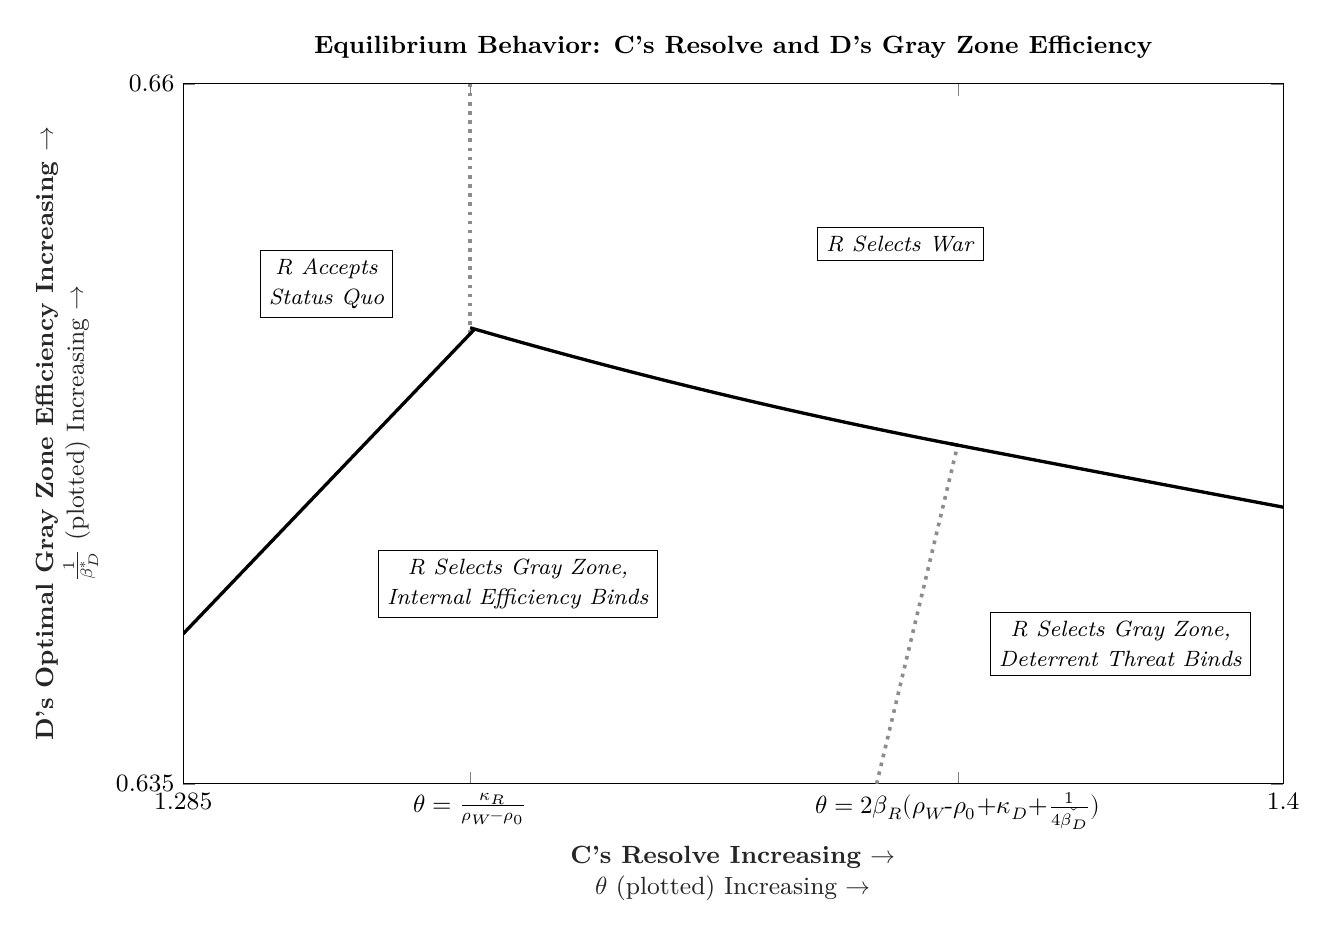
\begin{tikzpicture} 
\small
\begin{axis}[%
width=5.5in,
height=3.5in,
at={(1.011in,0.642in)},
scale only axis,
xmin=1.285,
xmax=1.4,
xtick={1.285, 1.315, 1.366,1.4},
xticklabels={{1.285},{$\theta=\frac{\kappa_R}{\rho_W-\rho_0}$},{$\theta=2\beta_R(\rho_{W}$-$\rho_{0}$+$\kappa_{D}$+$\frac{1}{4\check{\beta_D}})$},{1.4}},
%{\shortstack{$\frac{\theta}{2\beta}=(\rho_{W}-$\\$\rho_{0}+\kappa_{D}+\frac{d}{4})$}}
xlabel style={font=\color{white!15!black},align=center},
xlabel={\textbf{C's Resolve Increasing $\rightarrow$} \\ $\theta$ (plotted) Increasing $\rightarrow$ },
ymin=0.635,
ymax=0.67,
ytick={0.635, 0.67},
yticklabels={{0.635},{0.66}},
ylabel style={font=\color{white!15!black}, align=center},
ylabel={\textbf{D's Optimal Gray Zone Efficiency Increasing $\rightarrow$} \\ $\frac{1}{\beta_D^*}$ (plotted) Increasing $\rightarrow$},
axis background/.style={fill=white},
title style={font=\bfseries},
title={Equilibrium Behavior: C's Resolve and D's Gray Zone Efficiency},
]

%
 
\node[draw, align=center] at (1.3,0.66) {\footnotesize{\textit{R Accepts}} \\ \footnotesize{\textit{Status Quo}}};
\node[draw, align=center] at (1.32,0.645) {\footnotesize{\textit{R Selects Gray Zone,}} \\ \footnotesize{\textit{Internal Efficiency Binds}}}; 
\node[draw, align=center] at (1.383,0.642) {\footnotesize{\textit{R Selects Gray Zone,}} \\ \footnotesize{\textit{Deterrent Threat Binds}}}; 
\node[draw, align=center] at (1.36,0.662) {\footnotesize{\textit{R Selects War}}};  

%\node[draw, align=center] at (.1925,1.2) {\footnotesize{\textit{Gray Zone,}} \\ \footnotesize{\textit{Unconstrained}}}; 

%BEGIN DOTTED LINES

\addplot [color=white!55!black, dotted, line width=1.3pt, forget plot]
  table[row sep=crcr]{%
1.315   0.6575\\
1.315   0.67\\
};


%\addplot [color=white!55!black, dotted, line width=1.3pt, forget plot]
 % table[row sep=crcr]{%
%1.315  0.6575\\
%1.315  0.635\\
%};

%END DOTTED LINES

%WAR
%\addplot [color=black, line width=1.2pt]
%  table[row sep=crcr]{%
%1.315      0.6575\\
%1.315          0.69\\
%};

%GZ CONSTRAINTS
\addplot[color=white!55!black, dotted, line width=1.3pt, forget plot]
  table[row sep=crcr]{%
1.3575  0.635   \\
1.358   0.636   \\
1.3585  0.637   \\
1.359   0.638   \\
1.3595  0.639   \\
1.36    0.64    \\
1.3605  0.641   \\
1.361   0.642   \\
1.3615  0.643   \\
1.362   0.644   \\
1.3625  0.645   \\
1.363   0.646   \\
1.3635  0.647   \\
1.364   0.648   \\
1.3645  0.649   \\
1.365   0.65    \\
1.3655  0.651   \\
1.366   0.652   \\
};

%GZ INTERIOR PEACE
\addplot [color=black, line width=1.2pt, forget plot]
  table[row sep=crcr]{%
1.285   0.6425  \\
1.286   0.643   \\
1.287   0.6435  \\
1.288   0.644   \\
1.289   0.6445  \\
1.29    0.645   \\
1.291   0.6455  \\
1.292   0.646   \\
1.293   0.6465  \\
1.294   0.647   \\
1.295   0.6475  \\
1.296   0.648   \\
1.297   0.6485  \\
1.298   0.649   \\
1.299   0.6495  \\
1.3 0.65    \\
1.301   0.6505  \\
1.302   0.651   \\
1.303   0.6515  \\
1.304   0.652   \\
1.305   0.6525  \\
1.306   0.653   \\
1.307   0.6535  \\
1.308   0.654   \\
1.309   0.6545  \\
1.31    0.655   \\
1.311   0.6555  \\
1.312   0.656   \\
1.313   0.6565  \\
1.314   0.657   \\
1.315   0.6575  \\
1.3155  0.65775 \\
};

%GZ INTERIOR WAR
\addplot [color=black, line width=1.2pt, forget plot]
  table[row sep=crcr]{%
1.315   0.657804183 \\
1.316   0.657665653 \\
1.317   0.657528094 \\
1.318   0.657391502 \\
1.319   0.657255876 \\
1.32    0.657121212 \\
1.321   0.656987509 \\
1.322   0.656854766 \\
1.323   0.656722978 \\
1.324   0.656592145 \\
1.325   0.656462264 \\
1.326   0.656333333 \\
1.327   0.65620535  \\
1.328   0.656078313 \\
1.329   0.65595222  \\
1.33    0.655827068 \\
1.331   0.655702855 \\
1.332   0.65557958  \\
1.333   0.655457239 \\
1.334   0.655335832 \\
1.335   0.655215356 \\
1.336   0.655095808 \\
1.337   0.654977188 \\
1.338   0.654859492 \\
1.339   0.654742718 \\
1.34    0.654626866 \\
1.341   0.654511931 \\
1.342   0.654397914 \\
1.343   0.65428481  \\
1.344   0.654172619 \\
1.345   0.654061338 \\
1.346   0.653950966 \\
1.347   0.6538415   \\
1.348   0.653732938 \\
1.349   0.653625278 \\
1.35    0.653518519 \\
1.351   0.653412657 \\
1.352   0.653307692 \\
1.353   0.653203622 \\
1.354   0.653100443 \\
1.355   0.652998155 \\
1.356   0.652896755 \\
1.357   0.652796242 \\
1.358   0.652696613 \\
1.359   0.652597866 \\
1.36    0.6525  \\
1.361   0.652403012 \\
1.362   0.652306902 \\
1.363   0.652211665 \\
1.364   0.652117302 \\
1.365   0.65202381  \\
1.366   0.651931186 \\
};

%GZ External WAR
\addplot [color=black, line width=1.2pt, forget plot]
  table[row sep=crcr]{%
1.409290323 0.648   \\
1.408172501 0.6481  \\
1.40705556  0.6482  \\
1.405939499 0.6483  \\
1.404824316 0.6484  \\
1.40371001  0.6485  \\
1.402596581 0.6486  \\
1.401484027 0.6487  \\
1.400372347 0.6488  \\
1.399261541 0.6489  \\
1.398151606 0.649   \\
1.397042543 0.6491  \\
1.39593435  0.6492  \\
1.394827026 0.6493  \\
1.393720569 0.6494  \\
1.39261498  0.6495  \\
1.391510256 0.6496  \\
1.390406398 0.6497  \\
1.389303403 0.6498  \\
1.388201271 0.6499  \\
1.3871  0.65    \\
1.38599959  0.6501  \\
1.38490004  0.6502  \\
1.383801348 0.6503  \\
1.382703514 0.6504  \\
1.381606537 0.6505  \\
1.380510415 0.6506  \\
1.379415148 0.6507  \\
1.378320734 0.6508  \\
1.377227172 0.6509  \\
1.376134462 0.651   \\
1.375042603 0.6511  \\
1.373951592 0.6512  \\
1.372861431 0.6513  \\
1.371772116 0.6514  \\
1.370683648 0.6515  \\
1.369596025 0.6516  \\
1.368509247 0.6517  \\
1.367423312 0.6518  \\
1.36633822  0.6519  \\
1.365253968 0.652   \\
};


 
%   \node at (1.3,0.502)  [circle,scale=0.7,minimum size=0.5pt,draw,fill=black!100] {};
  %  \node at (1.3,0.65)  [circle,scale=0.7,draw,fill=black!0] {};


            


\end{axis}
\end{tikzpicture}\vspace{0.8cm}

\caption{Extension 1: D's Optimal $d^{*}$}
\caption*{C's resolve $\theta$ and the inverse D's gray zone efficiency $\frac{1}{\beta_{D}}$ are plotted. The dotted lines separate different kinds of equilibrium play, and the dark black lines denote D's optimal selected $\beta_{D}$. The parameters are $\rho_{0}=0$, $\rho_{W}=0.5$, $\beta_{C}=1$, $\kappa_{C}=0.53$, and $\kappa_{D}=0.1$.}
\end{figure}

Moving left to right, for \(\theta\) between \(1.285\) and
\(\frac{\kappa_{C}}{\rho_{W}-\rho_{0}}\), D's optimal \(\beta_{D}^{*}\)
is described in Proposition A Case 1.A. As the outcome, C will optimally
select into the status quo. For this selected \(\beta_{D}^{*}\), C knows
that C would face enough of a challenge in gray zone conflict to make
competing there too costly. Thus within this region, D could select a
low enough \(\beta_{D}^{*}\) to compel C to forgo limited challenges and
conflict, and stick to the status quo.\textbackslash{} \textbackslash{}
Moving right, for \(\theta\) between
\(\frac{\kappa_{C}}{\rho_{W}-\rho_{0}}\) and
\(\ensuremath{2\beta_{C}(\rho_{W}-\ensuremath{\rho_{0}}+\kappa_{D}}+\frac{1}{4\check{\beta_{D}}})\),
D's optimal \(\beta_{D}^{*}\) is described in Proposition A Case 2.A. As
the outcome, C will optimally select into gray zone conflict, but will
be constrained by C's internal costs. For this selected
\(\beta_{D}^{*}\), D wants to challenge C in gray zone conflict (which a
lower \(\beta_{D}^{*}\) accomplishes), but does not want to push C into
forgoing gray zone conflict, because within this region C prefers war to
accepting the status quo. Thus here, D selects the \(\beta_{D}^{*}\)
where C selects into gray zone conflict and is not bound by the
deterrent threat, because this gives D some surplus beyond what war or C
selecting gray zone conflict and being bound by the deterrent threat
produces.\textbackslash{} \textbackslash{} Finally, for \(\theta\)
between
\(\ensuremath{2\beta_{C}(\rho_{W}-\ensuremath{\rho_{0}}+\kappa_{D}}+\frac{1}{4\check{\beta_{D}}})\)
and \(1.4\), D's optimal \(\beta_{D}^{*}\) is described in Case 2.B. As
the outcome, C will optimally select into gray zone conflict, and will
be constrained by D's deterrent threat. Essentially here, D is in a bad
situation. If D modifies \(\beta_{D}^{*},\)either C will adapt by
selecting the new \(g_{C}^{*}\) that makes D indifferent between war and
gray zone conflict, or will go to war over the issue. Within this
region, it does not matter what \(\beta_{D}^{*}\) is selected, because C
will always select an action that gives D their wartime utility.

\hypertarget{extension-2-probabilistic-escalation-to-war}{%
\subsection{Extension 2: Probabilistic Escalation to
War}\label{extension-2-probabilistic-escalation-to-war}}

A useful feature of the model above is that everything that occurs is
deterministic. It is only if a state wants to go to war or wants to
enter gray zone conflict does it actually happen. However, this may not
perfectly represent reality. Perhaps in some cases, one state behaving
aggressively in lower-levels of conflict can create an incident that
necessitates an escalation to higher levels of conflict. To speak to
this issue, we introduce the possibility of probabilistic escalation out
of gray zone conflict. Our results are substantively similar, but this
change shifts some equilibrium properties. Intuitively, now gray zone
conflict can probabilistically lead to C's worst outcome: where C
invests in limited challenges, war happens, and C must pay the costs of
limited challenges with the costs of war. Strategically, because here
gray zone conflict is overall worse for R, C will be more willing to
accept the status quo or go to war.\textbackslash{} \textbackslash{}
There are many possible ways to model this. For ease, we choose (in our
opinion) the simplest way, which is that selecting \(g_{C}>0\)
introduces a \(1-\zeta\in(0,1)\) likelihood of an escalation to war.
Thus, when C selects \(g_{C}>0\), C's new expected utility is
\begin{align*}
U_{C}= & \theta\left(\zeta P(g_{C},g_{D})+(1-\zeta)\rho_{W}\right)-(1-\zeta)\kappa_{C}-\beta_{C}g_{C}.
\end{align*} To offer some intuition, \(g_{D}^{*}\), \(\hat{g_{C}}\),
\(\check{g_{C}}\), and \(\tilde{g_{C}}\) remain the same as it was in
the model in the text (as defined in Proposition 1). However, the
cut-points that distinguish C's decision to enter into the status quo,
gray zone conflict, or war change slightly; overall, the key take-away
is that considering probabilistic escalation makes gray zone conflict
less appealing relative to the status quo and war.\textbackslash{}
\textbackslash{} I express equilibrium behavior in Proposition B. Then
below, I derive the new cut-points, Additionally in the derivations, I
discuss how the new cut-points imply that gray zone conflict is less
appealing and fewer types \(\theta\) will select into it relative to the
game without a probabilistic likelihood of escalation to war from gray
zone conflict. \textbackslash{} \textbackslash{}
\textbf{\textit{Proposition B:}}\textit{ In equilibrium, the game with a $1-\zeta$ chance of escalation out of gray zone conflict to war will play out in the following manner.}\textbackslash{}
\textbackslash{}
\textit{Case 1, $\frac{\theta}{2\beta_{C}}\geq\rho_{W}-\rho_{0}+\kappa_{D}+\frac{1}{4\beta_{D}}$:}

\begin{itemize}
\item \textit{1.A. If $\theta\leq\frac{(1-\zeta)\kappa_{C}+\beta_{C}\left(\rho_{W}-\rho_{0}+\kappa_{D}+\frac{1}{4\beta_{D}}\right)^{2}}{(1-\zeta)(\rho_{W}-\rho_{0})+\zeta\left(\rho_{W}-\rho_{0}+\kappa_{D}-\frac{1}{4\beta_{D}}\right)}$ and $\theta\leq\frac{\kappa_{C}}{\rho_{W}-\rho_{0}}$, then C accepts the status quo. C selects $w_{R}^{*}=0$ and $g_{C}^{*}=0$, and D selects $w_{D}^{*}=0$ and $g_{D}^{*}=0$. } 
\item \textit{1.B. If $\theta>\frac{\zeta\kappa_{C}-\beta_{C}\left(\rho_{W}-\rho_{0}+\kappa_{D}+\frac{1}{4\beta_{D}}\right)^{2}}{\zeta\left(\frac{1}{4\beta_{D}}-\kappa_{D}\right)}$ and $\theta>\frac{\kappa_{C}}{\rho_{W}-\rho_{0}}$, then C declares war. C selects $w_{R}^{*}=1$.} 
\item \textit{1.C. Otherwise, the game end in gray zone conflict where }C's\textit{ limited challenge is constrained by D's deterrent threat. C selects $w_{R}^{*}=0$ and $g_{C}^{*}=\rho_{W}-\rho_{0}+\kappa_{D}+\frac{1}{4\beta_{D}}$, and (assuming the game does not probabilistically escalate to war) D selects $w_{D}^{*}=0$ and $g_{D}^{*}=\frac{1}{2\beta_{D}}$. } 
\end{itemize}

\textit{Case 2, $\frac{\theta}{2\beta_{C}}<\rho_{W}-\rho_{0}+\kappa_{D}+\frac{1}{4\beta_{D}}$:}

\begin{itemize}
\item \textit{2.A. If $(1-\zeta)\kappa_{C}\geq\theta\left((1-\zeta)(\rho_{W}-\rho_{0})+\zeta\left(\frac{\theta}{2\beta_{C}}-\frac{1}{2\beta_{D}}\right)-\frac{\theta}{4\beta_{C}}\right)$ and $\theta\leq\frac{\kappa_{C}}{\rho_{W}-\rho_{0}}$, then C accepts the status quo. C selects $w_{R}^{*}=0$ and $g_{C}^{*}=0$, and D selects $w_{D}^{*}=0$ and $g_{D}^{*}=0$. } 
\item \textit{2.B. If $\theta>\frac{\zeta\kappa_{C}}{\left(\zeta\left(\rho_{W}-\rho_{0}-\frac{\theta}{2\beta_{C}}+\frac{1}{2\beta_{D}}\right)+\frac{\theta}{4\beta_{C}}\right)}$ and $\theta>\frac{\kappa_{C}}{\rho_{W}-\rho_{0}}$, then C declares war. C sets $w_{R}^{*}=1$.}\footnote{\textit{While the right-hand-side of this condition is also increasing in $\theta$, by Assumption 2, the left-hand-side increases faster with increases in $\theta$.}}\textit{ } 
\item \textit{2.C. Otherwise, the game will end in gray zone conflict where }C's\textit{ limited challenge is constrained by }C's\textit{ internal efficiency. C selects $w_{R}^{*}=0$ and $g_{C}^{*}=\frac{\theta}{2\beta_{C}}$, and (assuming the game does not probabilistically escalate to war) D selects $w_{D}^{*}=0$ and $g_{D}^{*}=\frac{1}{2\beta_{D}}$. } 
\end{itemize}

\hypertarget{equilibrium-intuation}{%
\subsubsection{Equilibrium Intuation}\label{equilibrium-intuation}}

First, we consider the case when
\(\frac{\theta}{2\beta_{C}}\geq\rho_{W}-\rho_{0}+\kappa_{D}+\frac{1}{4\beta_{D}}\).
This implies that C will select
\(g_{C}^{*}=\hat{g_{C}}=\rho_{W}-\rho_{0}+\kappa_{D}+\frac{1}{4\beta_{D}}\).
We can then express C's behavior in terms of \(\theta\). C prefers the
status quo to gray zone conflict when \begin{align*}
\theta\rho_{0}\geq & \theta\left(\zeta\left(\rho_{W}+\kappa_{D}-\frac{1}{4\beta_{D}}\right)+(1-\zeta)\rho_{W}\right)-(1-\zeta)\kappa_{C}-\beta_{C}\left(\rho_{W}-\rho_{0}+\kappa_{D}+\frac{1}{4\beta_{D}}\right)^{2}
\end{align*} or \begin{align*}
\frac{\beta_{C}\left(\rho_{W}-\rho_{0}+\kappa_{D}+\frac{1}{4\beta_{D}}\right)^{2}}{\zeta\left(\rho_{W}-\rho_{0}+\kappa_{D}-\frac{1}{4\beta_{D}}\right)}+\frac{(1-\zeta)(\theta\rho_{0}-\theta\rho_{W}+\kappa_{C})}{\zeta\left(\rho_{W}-\rho_{0}+\kappa_{D}-\frac{1}{4\beta_{D}}\right)}\geq & \theta.
\end{align*} Note that the inequality sign does not flip because, by
Assumption 1, \(\rho_{W}-\rho_{0}+\kappa_{D}-\frac{1}{4\beta_{D}}>0\). I
am able to say that
\(\frac{\beta_{C}\left(\rho_{W}-\rho_{0}+\kappa_{D}+\frac{1}{4\beta_{D}}\right)^{2}}{\zeta\left(\rho_{W}-\rho_{0}+\kappa_{D}-\frac{1}{4\beta_{D}}\right)}>\frac{\beta_{C}\left(\rho_{W}-\rho_{0}+\kappa_{D}+\frac{1}{4\beta_{D}}\right)^{2}}{\left(\rho_{W}-\rho_{0}+\kappa_{D}-\frac{1}{4\beta_{D}}\right)}\)
because \(\zeta\in(0,1)\). Furthermore, this constraint (on when the
status quo is preferred to gray zone conflict) matters only when C
prefers the status quo to war, or when
\(\theta\rho_{0}-\theta\rho_{W}+\kappa_{C}\geq0\); this condition
implies
\(\frac{(1-\zeta)(\theta\rho_{0}-\theta\rho_{W}+\kappa_{C})}{\zeta\left(\rho_{W}-\rho_{0}+\kappa_{D}-\frac{1}{4\beta_{D}}\right)}\geq0\),
which means
\(\frac{\beta_{C}\left(\rho_{W}-\rho_{0}+\kappa_{D}+\frac{1}{4\beta_{D}}\right)^{2}}{\zeta\left(\rho_{W}-\rho_{0}+\kappa_{D}-\frac{1}{4\beta_{D}}\right)}+\frac{(1-\zeta)(\theta\rho_{0}-\theta\rho_{W}+\kappa_{C})}{\zeta\left(\rho_{W}-\rho_{0}+\kappa_{D}-\frac{1}{4\beta_{D}}\right)}>\frac{\beta_{C}\left(\rho_{W}-\rho_{0}+\kappa_{D}+\frac{1}{4\beta_{D}}\right)^{2}}{\left(\rho_{W}-\rho_{0}+\kappa_{D}-\frac{1}{4\beta_{D}}\right)}\),
which in turn implies that there are more C's with some resolve
\(\theta\) that will select into the status quo in the game here
relative to the game in the text without probabilistic
escalation.\textbackslash{} \textbackslash{} Next, C prefers war to gray
zone conflict when

\begin{align*}
\theta\rho_{W}-\kappa_{C}> & \theta\left(\zeta\left(\rho_{W}+\kappa_{D}-\frac{1}{4\beta_{D}}\right)+(1-\zeta)\rho_{W}\right)-(1-\zeta)\kappa_{C}-\beta_{C}\left(\rho_{W}-\rho_{0}+\kappa_{D}+\frac{1}{4\beta_{D}}\right)^{2}
\end{align*} or \begin{align*}
\theta> & \frac{\zeta\kappa_{C}-\beta_{C}\left(\rho_{W}-\rho_{0}+\kappa_{D}+\frac{1}{4\beta_{D}}\right)^{2}}{\zeta\left(\frac{1}{4\beta_{D}}-\kappa_{D}\right)}.
\end{align*} Note that based on Assumption 2 (as is written: that
\(\frac{1}{4\beta_{D}}-\kappa_{D}>0\)), the above sign does not flip. I
can say that
\(\zeta\kappa_{C}-\zeta\beta_{C}\left(\rho_{W}-\rho_{0}+\kappa_{D}+\frac{1}{4\beta_{D}}\right)^{2}>\zeta\kappa_{C}-\beta_{C}\left(\rho_{W}-\rho_{0}+\kappa_{D}+\frac{1}{4\beta_{D}}\right)^{2}\).
This implies that \{\footnotesize{} \begin{align*}
\frac{\kappa_{C}-\beta_{C}\left(\rho_{W}-\rho_{0}+\kappa_{D}+\frac{1}{4\beta_{D}}\right)^{2}}{\frac{1}{4\beta_{D}}-\kappa_{D}}=\frac{\zeta\kappa_{C}-\zeta\beta_{C}\left(\rho_{W}-\rho_{0}+\kappa_{D}+\frac{1}{4\beta_{D}}\right)^{2}}{\zeta\left(\frac{1}{4\beta_{D}}-\kappa_{D}\right)} & >\frac{\zeta\kappa_{C}-\beta_{C}\left(\rho_{W}-\rho_{0}+\kappa_{D}+\frac{1}{4\beta_{D}}\right)^{2}}{\zeta\left(\frac{1}{4\beta_{D}}-\kappa_{D}\right)}.
\end{align*} \}In other words, there are more C's with some resolve
\(\theta\) that will select into war in the game here relative to the
game without probabilistic escalation.\textbackslash{} \textbackslash{}
Next, I assume
\(\frac{\theta}{2\beta_{C}}<\rho_{W}-\rho_{0}+\kappa_{D}+\frac{1}{4\beta_{D}}\).
This condition implies that the selected gray zone conflict will be
constrained by C's internal costs and not D's deterrent threat. So, if C
selects into gray zone conflict, C will select
\(g_{C}^{*}=\check{g_{C}}=\frac{\theta}{2\beta_{C}}\). I can then
express C's behavior in terms of \(\theta\). C prefers the status quo to
gray zone conflict when \begin{align*}
\theta\rho_{0}\geq & \theta\left(\zeta\left(\rho_{0}+\frac{\theta}{2\beta_{C}}-\frac{1}{2\beta_{D}}\right)+(1-\zeta)\left(\rho_{W}\right)\right)-(1-\zeta)\kappa_{C}-\frac{\theta^{2}}{4\beta_{C}}
\end{align*} or \begin{align*}
(1-\zeta)\kappa_{C}\geq & \theta\left((1-\zeta)(\rho_{W}-\rho_{0})+\zeta\left(\frac{\theta}{2\beta_{C}}-\frac{1}{2\beta_{D}}\right)-\frac{\theta}{4\beta_{C}}\right).
\end{align*} To speak to this inequality, we will need to consider a few
different cases here.\textbackslash{} \textbackslash{} First, it could
be possible that
\(\left((1-\zeta)(\rho_{W}-\rho_{0})+\zeta\left(\frac{\theta}{2\beta_{C}}-\frac{1}{2\beta_{D}}\right)-\frac{\theta}{4\beta_{C}}\right)\leq0\).
When this is the case, then C would never want to select into gray zone
conflict as doing so would always be strictly worse for
R.\textbackslash{} \textbackslash{} Next, consider when
\(\left((1-\zeta)(\rho_{W}-\rho_{0})+\zeta\left(\frac{\theta}{2\beta_{C}}-\frac{1}{2\beta_{D}}\right)-\frac{\theta}{4\beta_{C}}\right)>0\)
and \((1-\zeta)(\theta\rho_{W}-\theta\rho_{0}-\kappa_{C})>0\). In this
case, C's wartime payoff \(\theta\rho_{W}-\kappa_{C}\) is greater than
C's status quo payoff, meaning that C would never select into the status
quo over selecting into war, meaning this constraint would never be
activated.\textbackslash{} \textbackslash{} Finally, consider when
\(\left((1-\zeta)(\rho_{W}-\rho_{0})+\zeta\left(\frac{\theta}{2\beta_{C}}-\frac{1}{2\beta_{D}}\right)-\frac{\theta}{4\beta_{C}}\right)>0\)
and \((1-\zeta)(\theta\rho_{W}-\theta\rho_{0}-\kappa_{C})<0\). I can
re-write the above as \begin{align*}
0\geq & \theta\left(\zeta\left(\frac{\theta}{2\beta_{C}}-\frac{1}{2\beta_{D}}\right)-\frac{\theta}{4\beta_{C}}\right)+(1-\zeta)(\theta\rho_{W}-\theta\rho_{0}-\kappa_{C})
\end{align*} Where note that
\(\frac{\theta}{4\beta_{C}}-\frac{1}{2\beta_{D}}=\frac{\theta}{2\beta_{C}}-\frac{1}{2\beta_{D}}-\frac{\theta}{4\beta_{C}}>\zeta\left(\frac{\theta}{2\beta_{C}}-\frac{1}{2\beta_{D}}\right)-\frac{\theta}{4\beta_{C}}\),
where the inequality holds by Assumption 1. Altogether, this means that
\(\text{\ensuremath{\theta\left(\frac{\theta}{4\beta_{C}}-\frac{1}{2\beta_{D}}\right)}}>\theta\left(\zeta\left(\frac{\theta}{2\beta_{C}}-\frac{1}{2\beta_{D}}\right)-\frac{\theta}{4\beta_{C}}\right)+(1-\zeta)(\theta\rho_{W}-\theta\rho_{0}-\kappa_{C})\).
This implies that there are more C's with some resolve \(\theta\) that
will select into the status quo in the game here relative to the game
without probabilistic escalation.\textbackslash{} \textbackslash{}
Finally, assuming
\(\frac{\theta}{2\beta_{C}}<\rho_{W}-\rho_{0}+\kappa_{D}+\frac{1}{4\beta_{D}}\),
C prefers war to gray zone conflict when \begin{align*}
\theta\rho_{W}-\kappa_{C}> & \theta\left(\zeta\left(\rho_{0}+\frac{\theta}{2\beta_{C}}-\frac{1}{2\beta_{D}}\right)+(1-\zeta)\left(\rho_{W}\right)\right)-(1-\zeta)\kappa_{C}-\frac{\theta^{2}}{4\beta_{C}}
\end{align*} or \begin{align*}
\theta> & \frac{\zeta\kappa_{C}}{\left(\zeta\left(\rho_{W}-\rho_{0}-\frac{\theta}{2\beta_{C}}+\frac{1}{2\beta_{D}}\right)+\frac{\theta}{4\beta_{C}}\right)}.
\end{align*} Note the inequality sign does not slip because
\(\left(\rho_{W}-\rho_{0}-\frac{\theta}{2\beta_{C}}+\frac{1}{2\beta_{D}}\right)>0\).
Furthermore, by that condition,
\(\zeta\left(\rho_{W}-\rho_{0}-\frac{\theta}{2\beta_{C}}+\frac{1}{2\beta_{D}}\right)+\frac{\theta}{4\beta_{C}}>\zeta\left(\rho_{W}-\rho_{0}-\frac{\theta}{2\beta_{C}}+\frac{1}{2\beta_{D}}\right)+\zeta\frac{\theta}{4\beta_{C}}\).
Therefore
\(\frac{\kappa_{C}}{\left(\rho_{W}-\rho_{0}-\frac{\theta}{2\beta_{C}}+\frac{1}{2\beta_{D}}\right)+\frac{\theta}{4\beta_{C}}}>\frac{\zeta\kappa_{C}}{\zeta\left(\rho_{W}-\rho_{0}-\frac{\theta}{2\beta_{C}}+\frac{1}{2\beta_{D}}\right)+\frac{\theta}{4\beta_{C}}}\).
This implies that there are more C's with some resolve \(\theta\) that
will select into war in the game here relative to the game without a
random chance of escalation.\textbackslash{} \textbackslash{} Finally,
note that D's strategies in this game are unchanged from the game
without probabilistic escalation.

\hypertarget{new-data}{%
\section{New data}\label{new-data}}

The universe of cases was created by first identifying cases of Russian
foreign interventions from 3 prior datasets; ICB, DCID, and REI. Code
replicating those findings is provided in the appropriate RMarkdown
files. These cases were then supplemented with additional cases of
Russian interference the authors were able to identify.

\hypertarget{coverage-of-current-datasets}{%
\subsection{Coverage of current
datasets}\label{coverage-of-current-datasets}}

A comparison of what cases were covered in each individual dataset is
provided here:
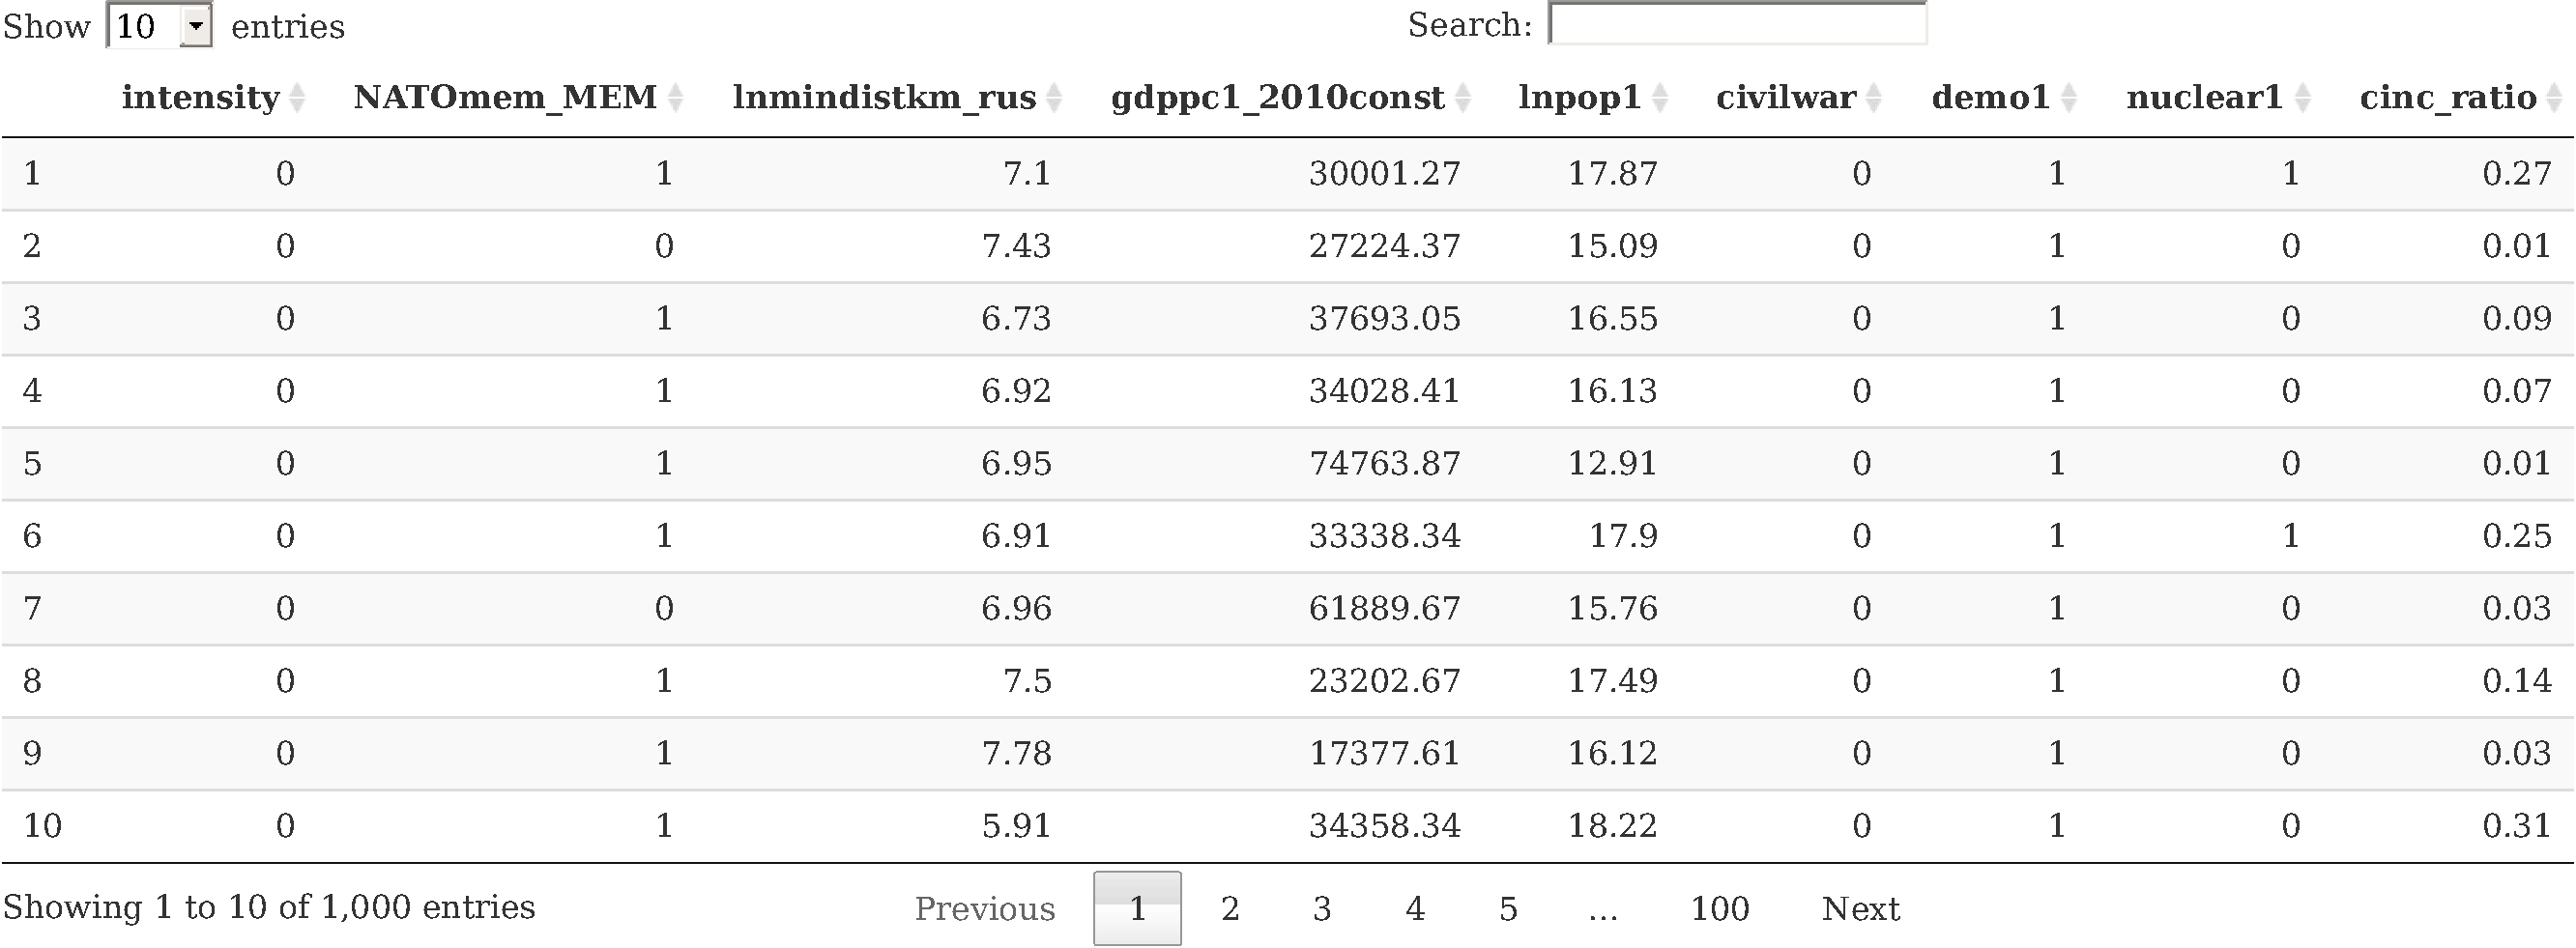
\includegraphics[width=4.50in,height=18.00in,keepaspectratio]{07_Appendix_files/figure-latex/unnamed-chunk-1-1.png}

The overlap between cases is seen here:
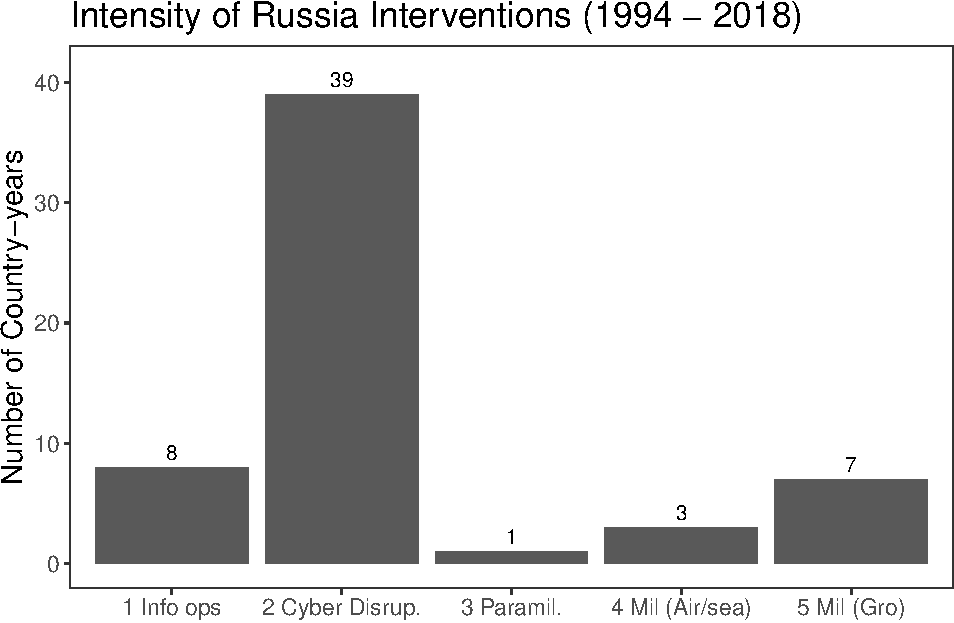
\includegraphics{07_Appendix_files/figure-latex/unnamed-chunk-2-1.pdf}

\hypertarget{consistency-of-current-datasets}{%
\subsection{Consistency of current
datasets}\label{consistency-of-current-datasets}}

Aside from the cases covered, the intensity codings for current datasets
are difficult to compare given their different scales. A more thorough
analysis is provided in the appropriate R Markdown files, but a
comparison of intensity codings in DCID (Valeriano and Maness) and REI
(Way and Casey) is visualized here:

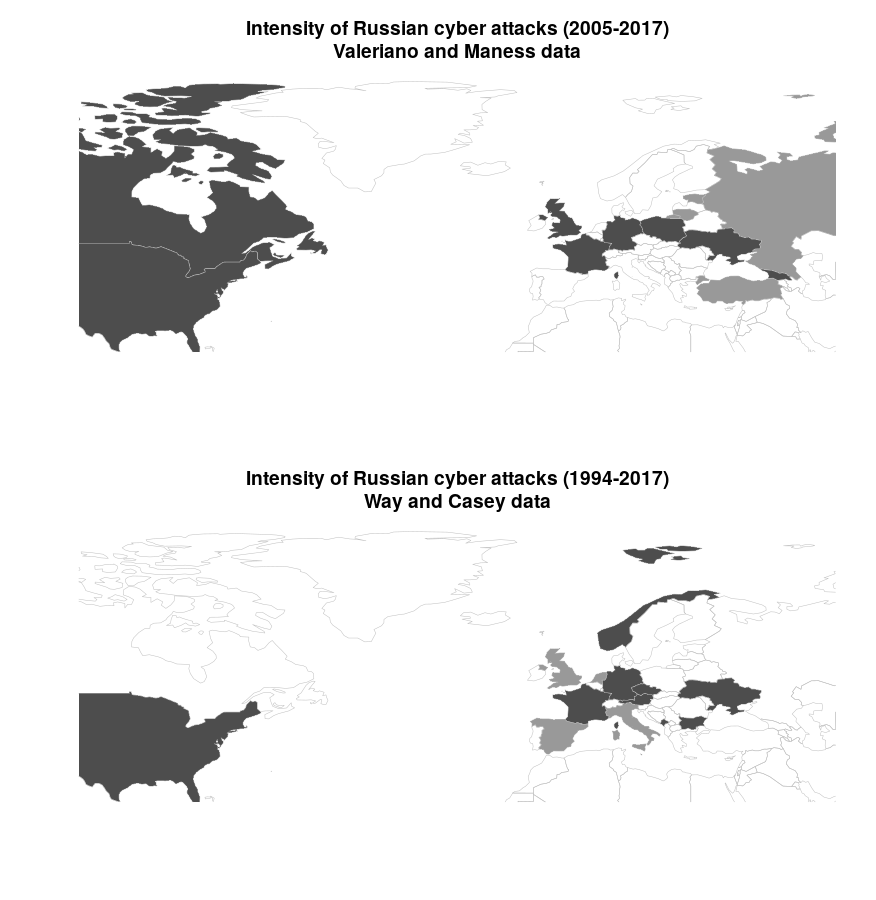
\includegraphics{../paper/figures/map_prior-data.png}

The DCID data identifies the United States, United Kingdom, Poland and
Ukraine as targets of the most severe Russian cyber operations. In the
cases documented by REI, the most severe Russian attacks occurred
against France, Austria, and Ukraine. Part of this discrepancy is due to
the respective foci of each dataset; DCID seeks out cases of cyber
incidents and disputes while REI focuses on Russian electoral
interference. While a majority of the REI cases include some form of
Russian cyber activity, there are a few cases where only material
support was provided (eg. Moldova 2014 and Belarus 1994). This
discrepancy exemplifies not only the challenges of relying on open
source reporting for identifying cyber influence or disruption
campaigns, but also differences in defining what counts as an attack.
The only country-year that appears in both datasets is Ukraine 2014. We
standardized codings across the two datasets using variable definitions
from respective codebooks. A severity less than or equal to 2 in DCID's
coding is synonymous in our recoding with REI's coding for
disinformation, a severity between 3 and 7 equals REI's coding for
cyberattack, and no cases in DCID have a severity greater than 7. We
adopted Valeriano and Maness (2014)'s approach of sampling on intensity
when there are multiple observations in a given time unit.

\hypertarget{variable-codings}{%
\subsection{Variable codings}\label{variable-codings}}

For each incident, we code whether Russia used conventional ground
forces, conventional air or sea forces, paramilitary or covert forces,
cyber disruption, and information operations. By distinguishing between
these five types of aggression, we obtain a clearer picture of the
intensity of each case of Russian intervention. The vast majority of
cases include at least some type of cyber operations. In a few cases,
data limitations preclude coding of non-kinetic activity by Russia or
other actors. In Moldova 2005, for example, Russia provided material
support for the Communist Party but there is no credible evidence of
cyber activities.

The following binary coding criteria were used for each case:

\begin{itemize}
\tightlist
\item
  \textbf{resp\_infoops} - Did Russia use information operations during
  this event? That includes propaganda, misinformation campaigns, etc
\item
  \textbf{resp\_cyberdisrup} - Did Russia use cyber attacks during this
  operation? That includes hacking, phishing, cyber espionage, DDOS
  attacks, etc
\item
  \textbf{resp\_paramil} - Did Russia use paramilitary troops during
  this event? Special forces, covert troops, speznatz, etc all count
\item
  \textbf{resp\_convmil\_airsea} - Did Russia use conventional naval or
  air forces during this event?
\item
  \textbf{resp\_convmil\_gro} - Did Russia use conventional ground
  troops like their army, artillery, tanks, etc during this event?
\end{itemize}

The complete dataset is provided in the appropriate .csv file. It
includes sources used for the codings as well as justifications and
explanations where needed.

\hypertarget{alternate-model-specifications}{%
\section{Alternate model
specifications}\label{alternate-model-specifications}}

\end{document}
